%--------------------------------------------------------------------------
% 	NEW SUBSECTION
%--------------------------------------------------------------------------
\section{Simulation vs schematic}
\subsection{Simulation setup}

\begin{frame}
	\tableofcontents[currentsubsection]
\end{frame}

\begin{frame}
\frametitle{Analysis}
	Developed analysis:
	\begin{itemize}
		\item Time domain output mixed signal and spectral components;
			\item Oscillator signal amplitude to maximize output component;
		\item Conversion gain and 1dB compression point;
		\item Single tone IIP\textsubscript{3};
		\item Two tone IIP\textsubscript{3};
		\item Bandwidth and CMRR of RF stage (output node filtering of output signal, current mixing);
		\item Static power dissipation;
	\end{itemize}
	Used frequencies: f\textsubscript{LO}=110MHz, f\textsubscript{RF}=100MHz, with expected f\textsubscript{IF}=10MHz.
\end{frame}

\begin{frame}
	\frametitle{Simulation setup}
	\begin{figure}[H]
		\centering %se si cambia posizione a questa immagine assicurarsi che sia girata con il fondo verso il bordo esterno della pagina
		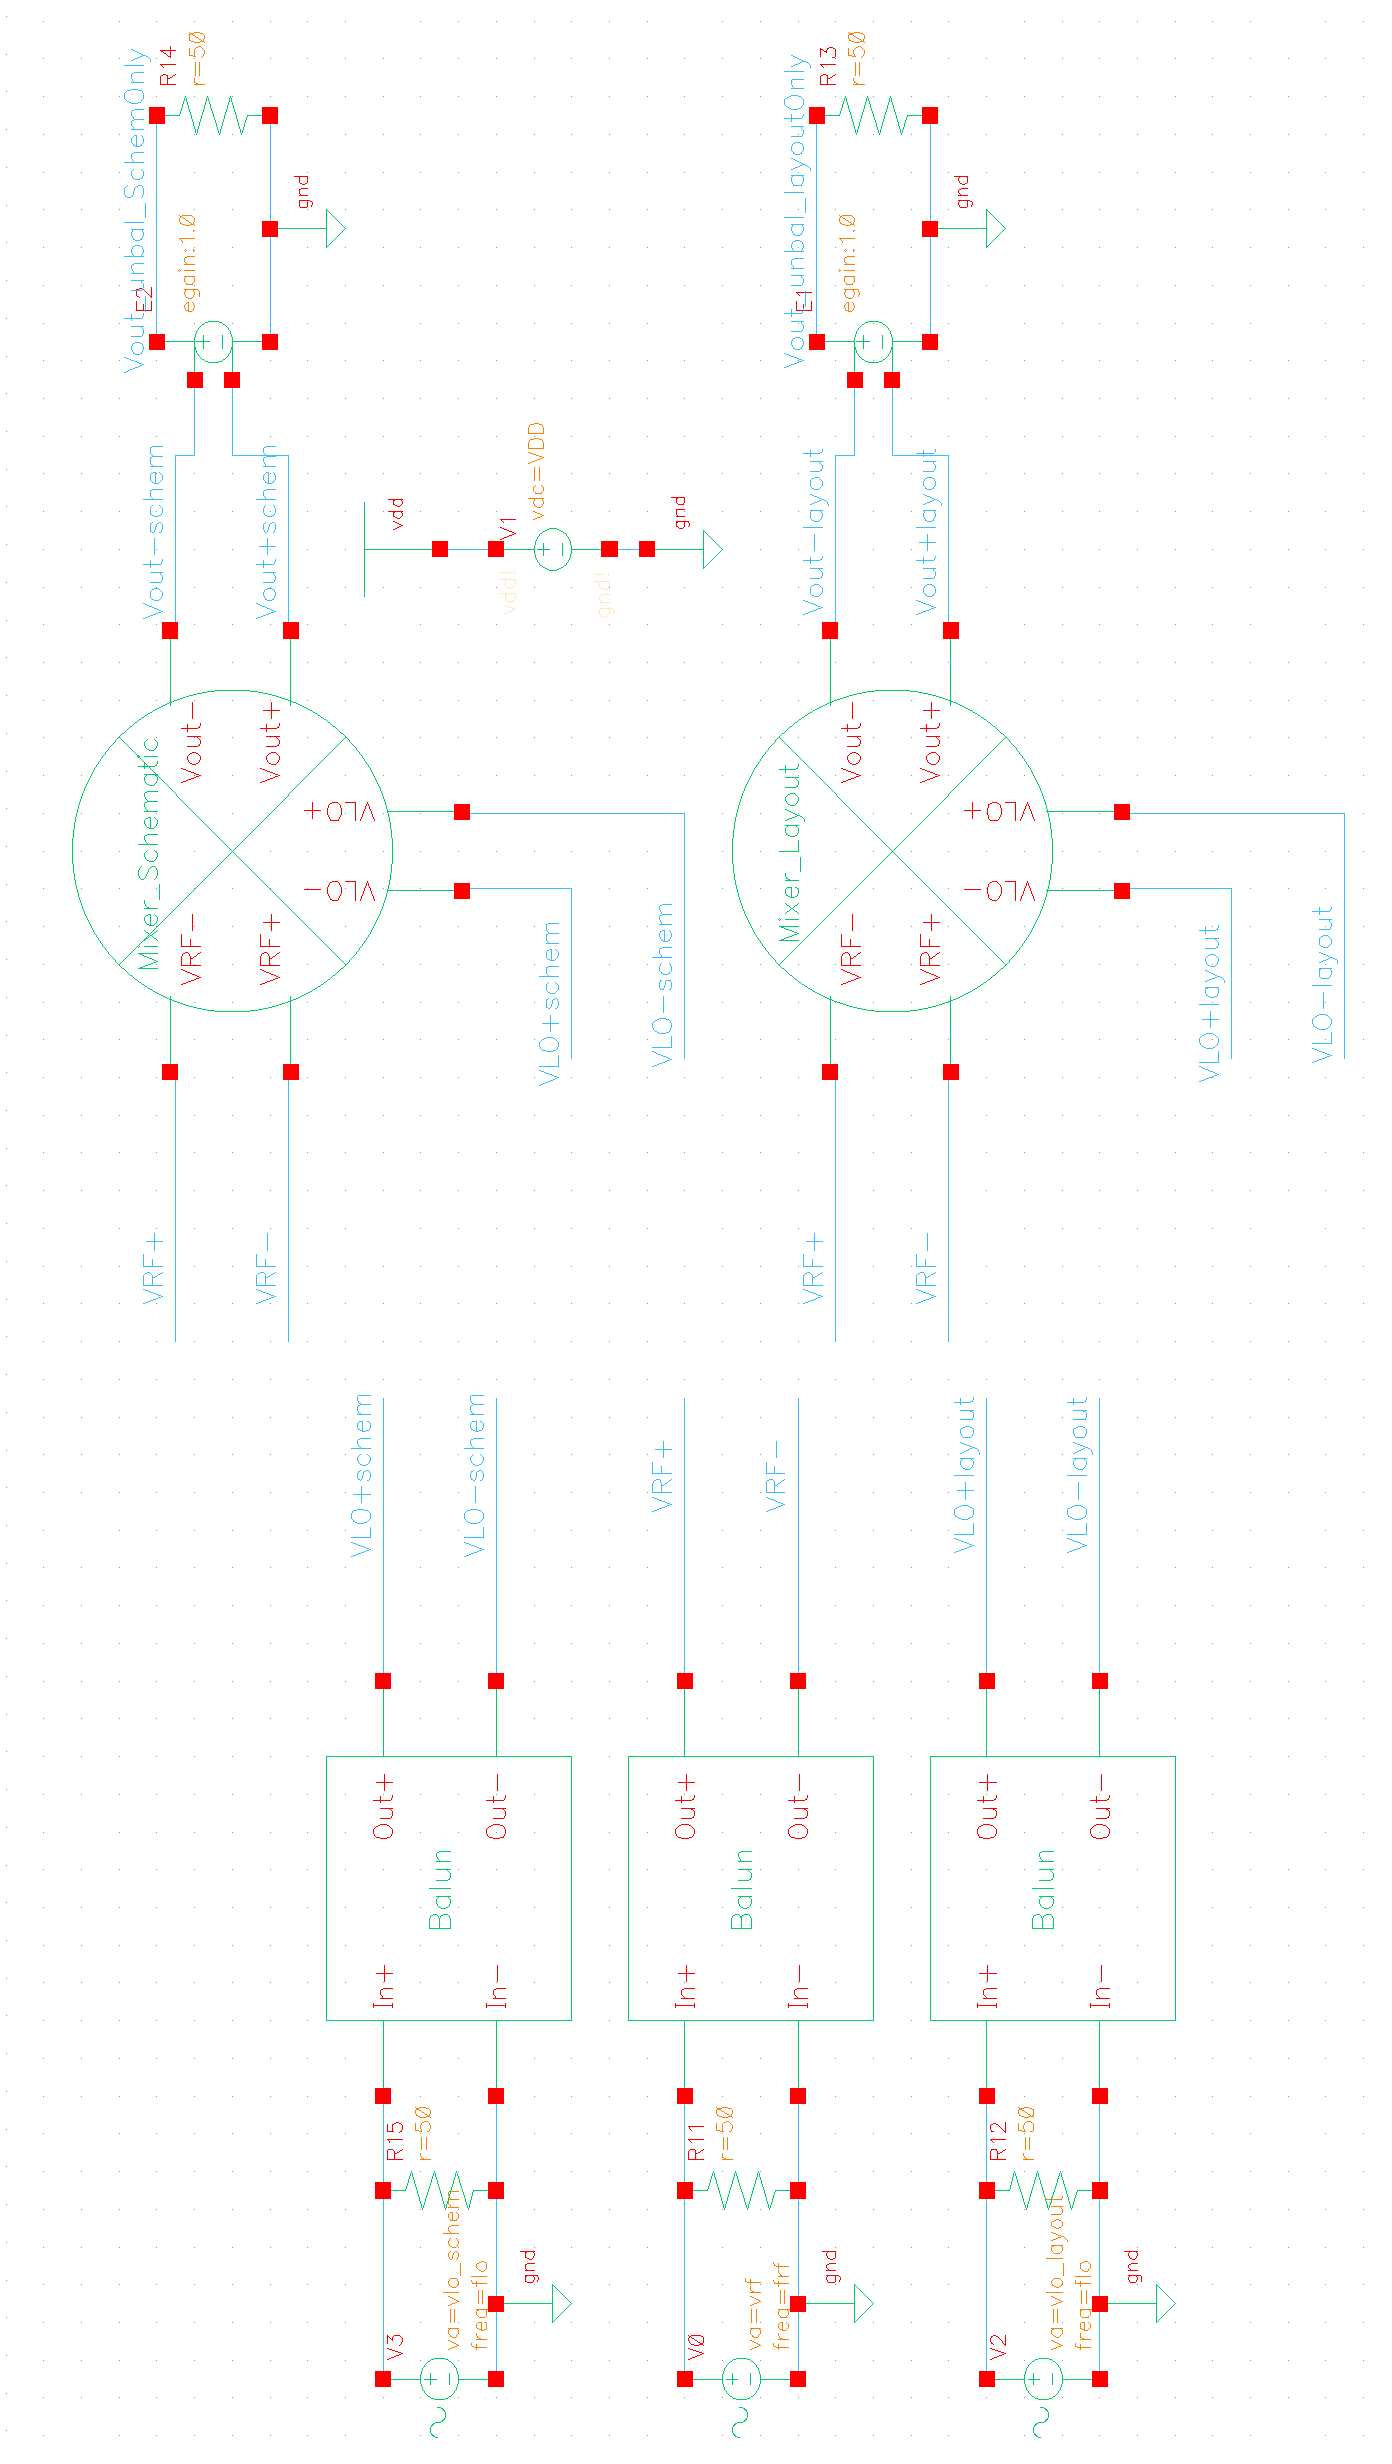
\includegraphics[scale=0.18, angle=-90]{setup}
		\label{fig:setup}
	\end{figure}
\end{frame}

\begin{frame}
	\frametitle{Simulation setup}
	\begin{figure}[H]
		\centering
		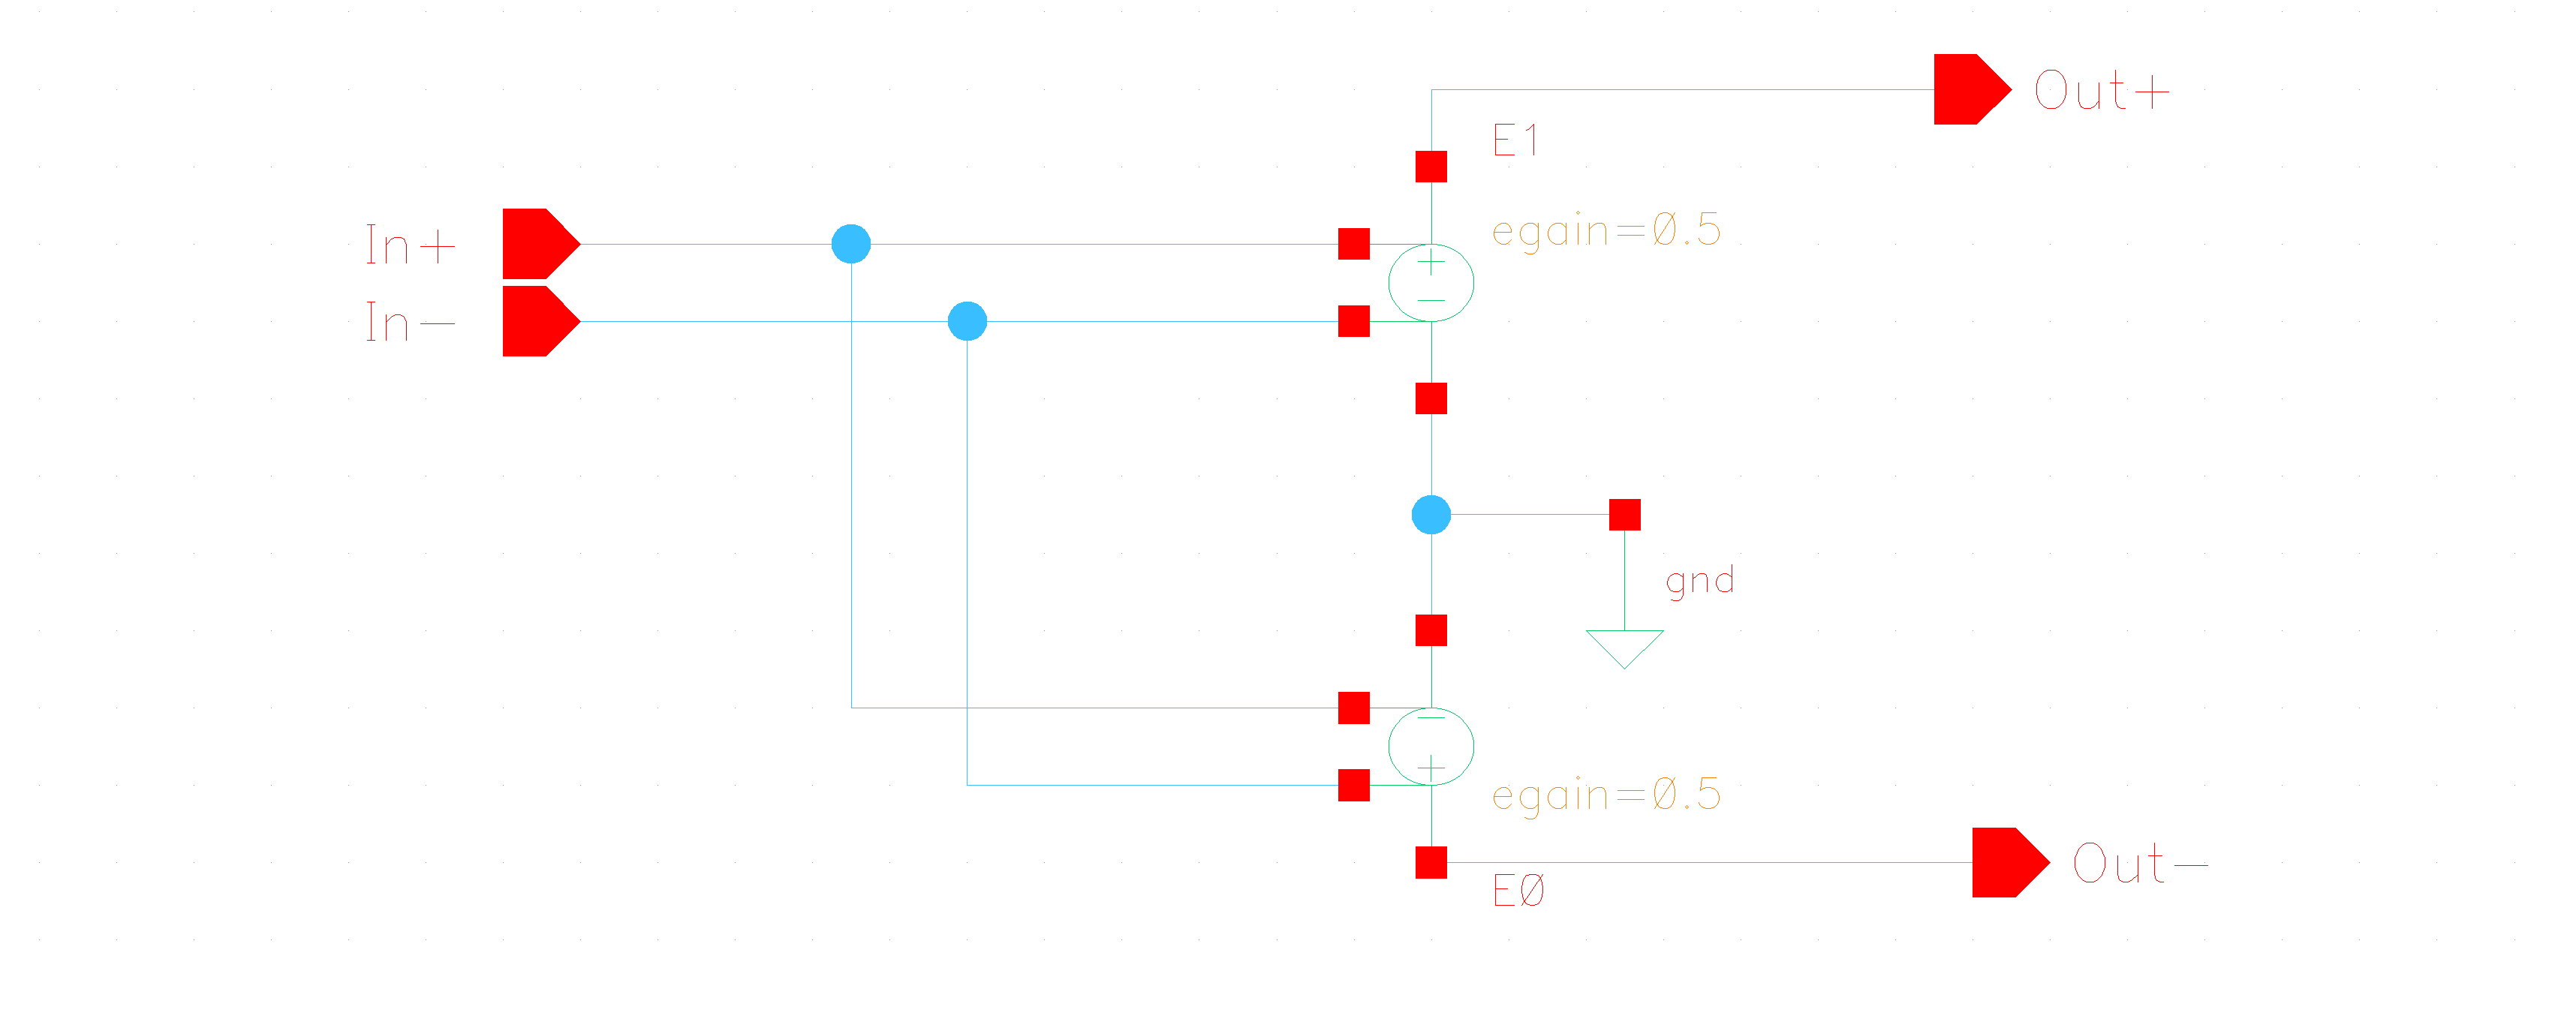
\includegraphics[scale=0.05]{balun}
		\caption{Balun schematic.}
		\label{fig:balun}
	\end{figure}
	\begin{itemize}
		\item Ideal baluns simulate a  50 \(\Omega\) impedance matching condition and produce differential inputs. 
		\item Power supply net, implicitly connected to both layout and schematic.
		\item Mixer's loads, represented by 50\(\Omega\) resistors connected to unitary gain driven generator. Used both for ideal impedance matching purposes and to convert differential output from mixers to single-ended.
	\end{itemize}
\end{frame}

%--------------------------------------------------------------------------
% 	NEW SUBSECTION
%--------------------------------------------------------------------------
\subsection{Time and frequency domain analysis}
\begin{frame}
\tableofcontents[currentsubsection]
\end{frame}

\begin{frame}
	\frametitle{Bandwidth evaluation - Transition frequency}
	Dynamic analysis is complex when dealing with non-linear circuits. The following results try to qualify the circuit in the best way.
	Always monochromatic signals have been used. 
\end{frame}

\begin{frame}
	\frametitle{Bandwidth evaluation - Transition frequency}
	\begin{columns}
	\column{0.4\textwidth}
	Maximum working frequency must be at least one decade below MOSFET transition frequency f\textsubscript{T}.
	From current gain measurements on M\textsubscript{3} and M\textsubscript{6}:
	\begin{gather}
		f_T|_{RF}=9.43GHz \notag \\
		f_T|_{LO}=1.12GHz \notag 
	\end{gather}  
	\column{0.6\textwidth}
	\begin{figure}[H]
		\centering 
		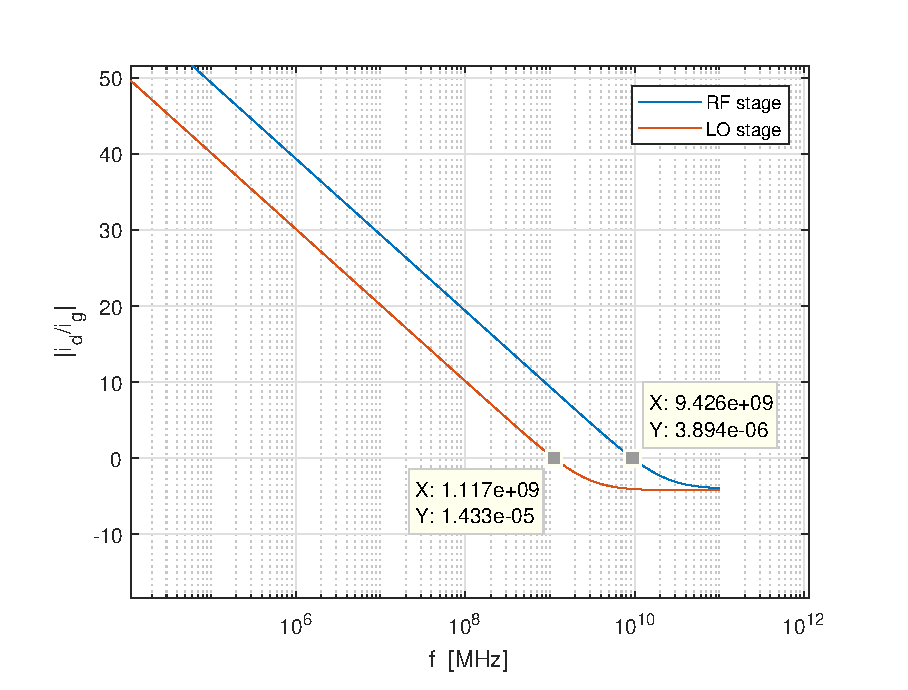
\includegraphics[scale=0.5]{transition_freq}
		\label{fig:ft}
	\end{figure}
	\end{columns}
\end{frame}

\begin{frame}
\frametitle{Bandwidth evaluation - Transition frequency}
\begin{columns}
	\column{0.4\textwidth}
	Bandwidth evaluated by plotting conversion gain dependency on frequency.
	The simulation is performed keeping \(f_{LO}=f_{RF}-10\)MHz.
	-3dB point is located almost two octaves above the maximum operation frequency.
	
	\column{0.6\textwidth}
	\begin{figure}[H]
		\centering 
		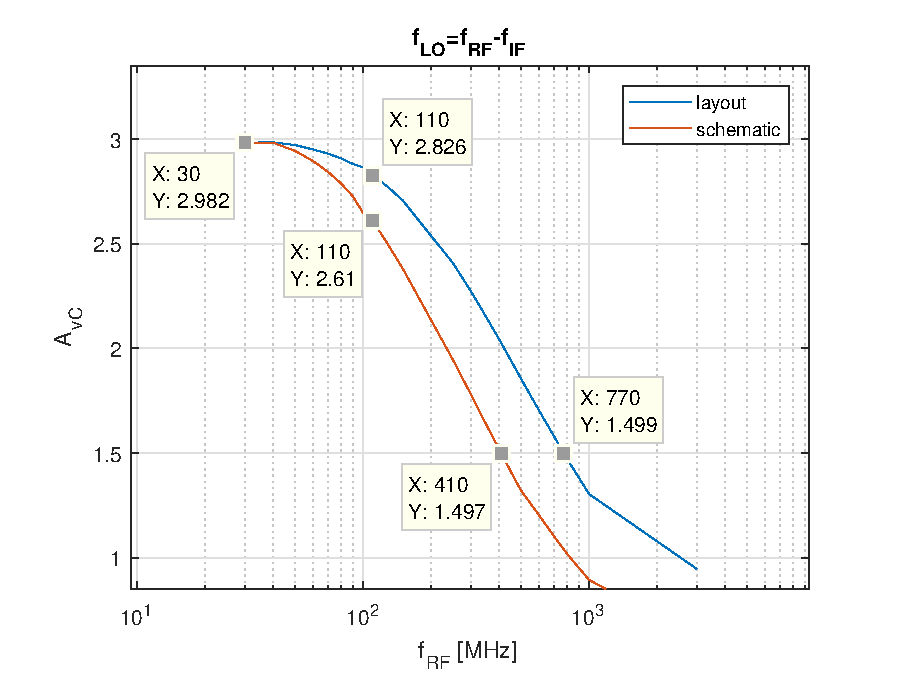
\includegraphics[scale=0.5]{bandwidth}
		\label{fig:band}
	\end{figure}
\end{columns}
\end{frame}

\begin{frame}
	\frametitle{Bandwidth evaluation - Conclusions}
	It is important to notice that we \textbf{cannot rely on this results} because:
	\begin{itemize}
		\item The technology kit is probably not suited for RF operation;
		\item The layout extraction does not account for all device and circuit parasitics, that would affect the performances at high frequency. The physical implementation would  probably not work;
		\item Pretending that results are accurate the simulation emulate the worst case operative condition. 
	\end{itemize}
\end{frame}

\begin{frame}
\frametitle{Max gain vs LO}
\begin{columns}
	\column{0.4\textwidth}
	LO level must be optimized to get maximum conversion gain. RF power is kept constant, sweeping pump input power.
	
	Layout seems to have better performance than schematic in term of maximum gain. From simulation:
	\begin{align}
	&V_{LO,opt}|_{layout}=1.23V \notag \\
	&V_{LO,opt}|_{schematic}=2.5V \notag
	\end{align}
	\column{0.6\textwidth}
	\begin{figure}[H]
		\centering
		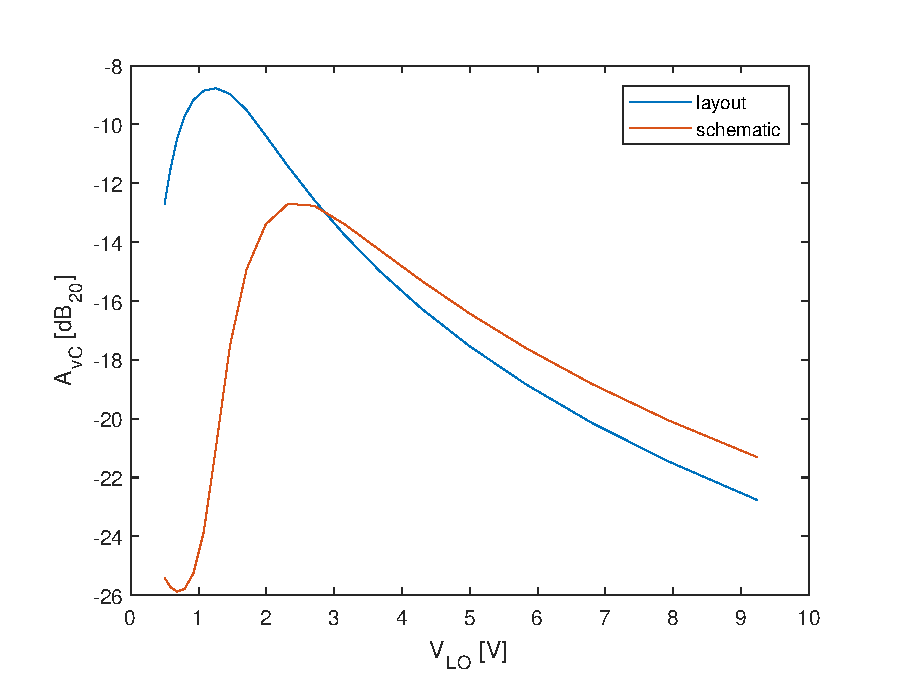
\includegraphics[scale=0.5]{gain_vs_VLO}
		\label{fig:maxGainvsLO}
	\end{figure}
\end{columns}
\end{frame}

\begin{frame}
\frametitle{Time domain analysis}
\begin{columns}
	\column{0.4\textwidth}
	It is possible to have a qualitative analysis about the distortion introduced by the circuit (detailed treatise later), by looking at the dft of the mixer's output signal. 
	\column{0.6\textwidth}
	\begin{figure}[H]
		\centering
		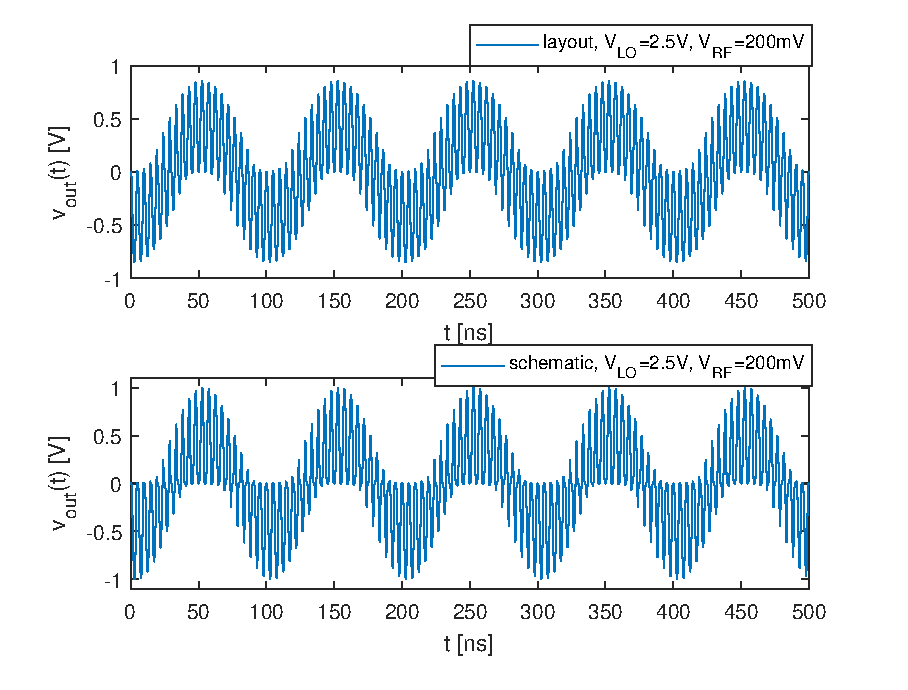
\includegraphics[scale=0.4]{waveforms}
		\caption{Time domain waveforms: double balanced differential output with v\textsubscript{RF}=200mV,  f\textsubscript{RF}=110MHz, v\textsubscript{RF}=1.23mV, f\textsubscript{LO}=100MHz.}
		\label{fig:TdomaniWF}
	\end{figure}
\end{columns}
\end{frame}

\begin{frame}
\frametitle{Output signal spectrum}
	\begin{figure}[H]
		\centering
		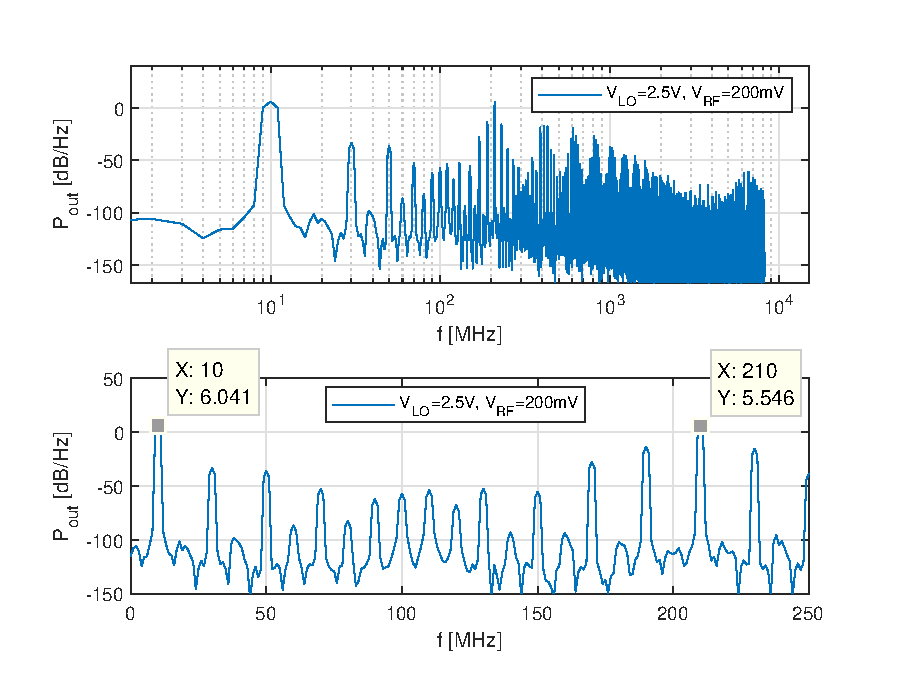
\includegraphics[scale=0.5]{DFT_layout}
		\caption{\textbf{Layout}. Discrete Fourier transform: double balanced differential output with v\textsubscript{RF}=200mV,  f\textsubscript{RF}=110MHz, v\textsubscript{RF}=1.23mV, f\textsubscript{LO}=100MHz,cosine squared smoothing function.}
	\end{figure}
\end{frame}

\begin{frame}
\frametitle{Output signal spectrum}
	\begin{figure}[H]
	\centering
	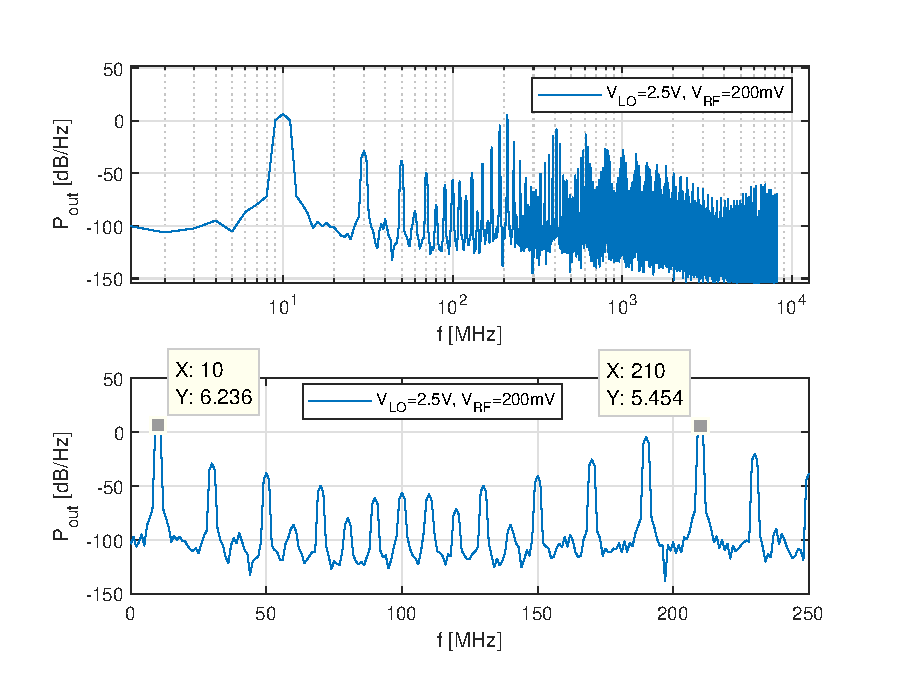
\includegraphics[scale=0.5]{DFT_schem}
	\caption{\textbf{Schematic}. Discrete Fourier transform: double balanced differential output with v\textsubscript{RF}=200mV,  f\textsubscript{RF}=110MHz, v\textsubscript{RF}=1.23mV, f\textsubscript{LO}=100MHz,cosine squared smoothing function.}
	\end{figure}
\end{frame}

\subsection{Power parameters}
\begin{frame}
\tableofcontents[currentsubsection]
\end{frame}

\begin{frame}
\frametitle{Conversion gain before compression}
\begin{columns}
\column{0.3\textwidth}
Given optimum $V_{LO}=1.23V$, RF voltage was swept to evaluate conversion gain before compression. Obtained conversion gains are as in figure:
\begin{gather}
A_{vC}|_{layout}=2.926 \notag \\ 
A_{vC}|_{schematic}=2.675 \notag
\end{gather}
\column{0.7\textwidth}
\begin{figure}[H]
	\centering
	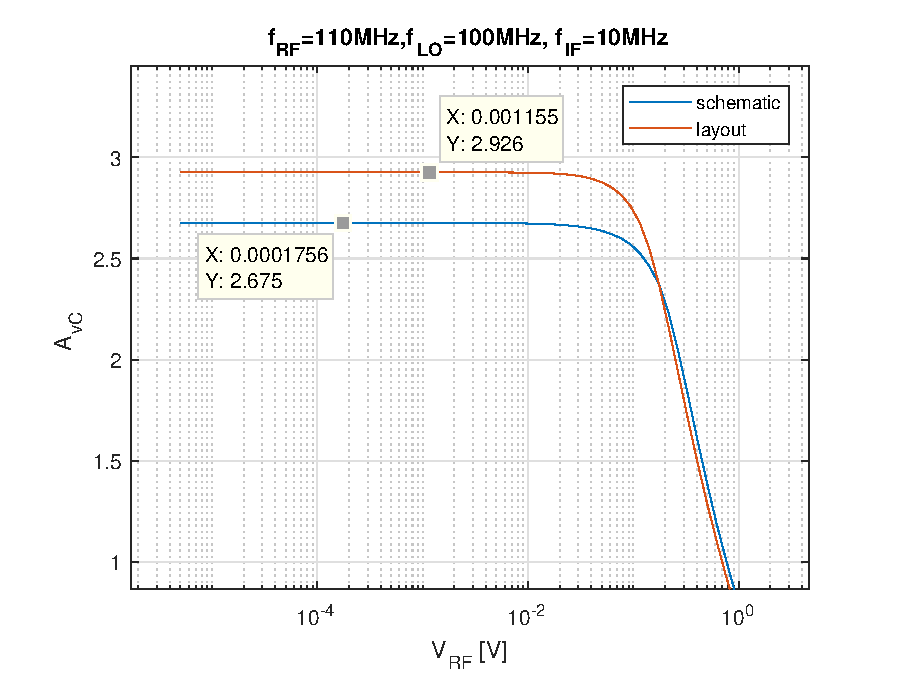
\includegraphics[width=\textwidth]{gain_vs_VRF}
	\caption{Conversion gain vs v\textsubscript{RF}}
	\label{fig:GainvsRF}
\end{figure}
\end{columns}
\end{frame}


\begin{frame}
\frametitle{Single tone $P_{in}$ $P_{out}$}
\begin{columns}
	\column{0.3\textwidth}
	All power measurements were carried on considering 50$\Omega$ reference impedance. Single tone $P_{in}$ $P_{out}$ for layout and schematic is visible in figure.
	\column{0.7\textwidth}
	\begin{figure}[H] 
		\centering
		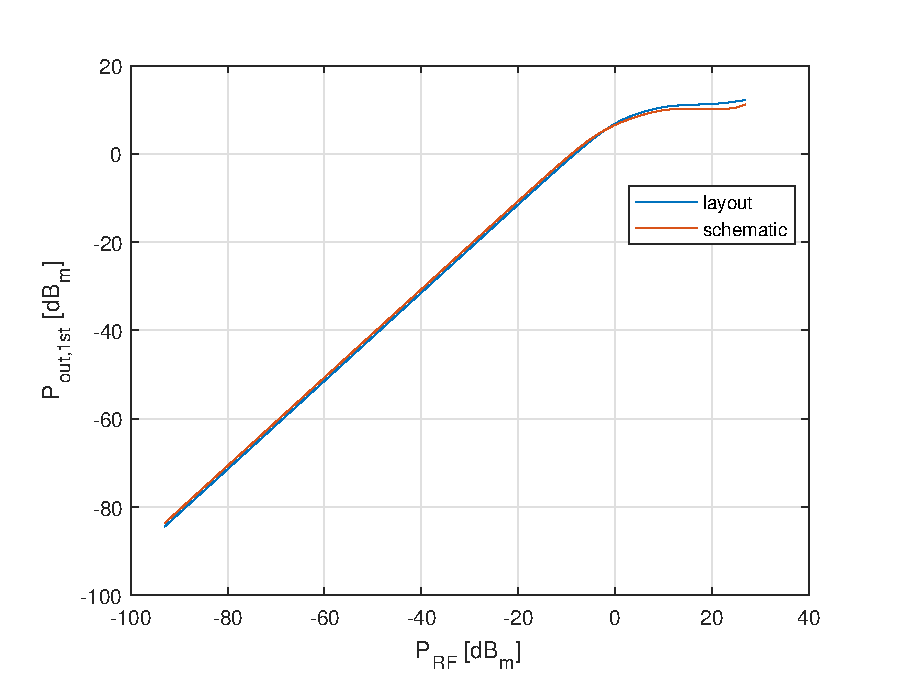
\includegraphics[width=\textwidth]{pin_pout_VRF}
		\caption{ P\textsubscript{in}/P\textsubscript{out}}
		\label{fig:PinPout}
	\end{figure}
\end{columns}
\end{frame}

\begin{frame}
\frametitle{1dB compression points}
\begin{columns}
	\column{0.3\textwidth}
	1dB compression point is defined as the input power for which output power decreases of 1dB with respect to non-compressed output power. A zoom-in of compression zone is visible in figure, with 1dB compression values highlighted.
	\column{0.7\textwidth}
	\begin{figure}[H] 
		\centering
		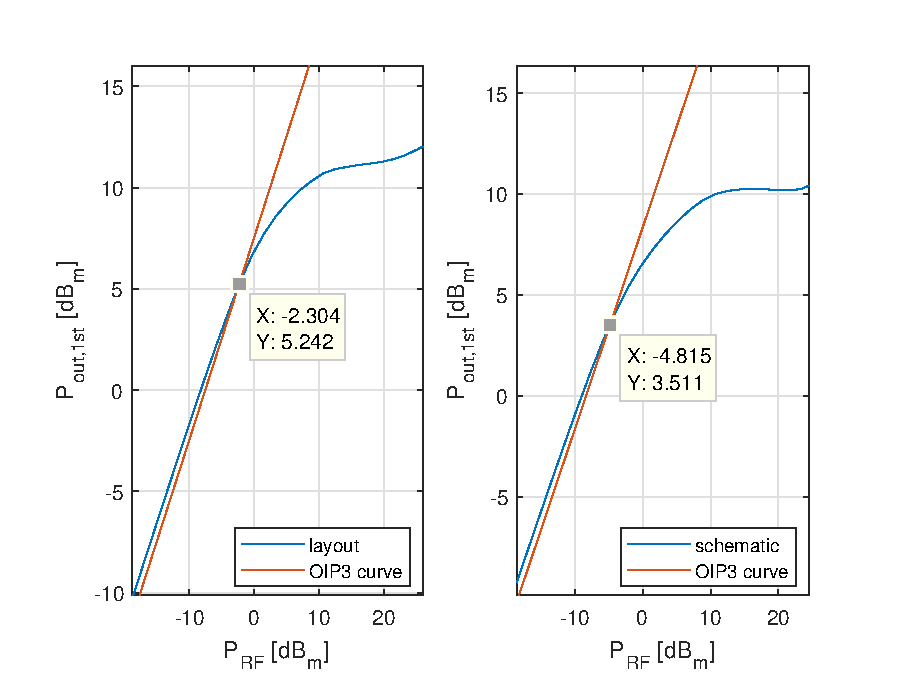
\includegraphics[width=\textwidth]{1dB_compression_1tone}
		\caption{ P\textsubscript{1dB compression point, one-tone analysis}}
		\label{fig:PinPout1T_1dBCp}
	\end{figure}
	\end{columns}
\end{frame}

\begin{frame}
\frametitle{1dB compression points}
\begin{columns}
	\column{0.4\textwidth}
	RF power for which gains drops of 1dB are equal to 
	\begin{gather}
	P_{RF,in}|_{layout}=-2.304dB_{m} \notag \\
	P_{RF,in}|_{schematic}=-4.815dB_{m} \notag
	\end{gather}
	then, respectively for schematic and layout, the corresponding voltages:
	\begin{gather}
	V_{RF,in}|_{layout}=172mV \notag \\
	V_{RF,in}|_{schematic}=128mV \notag
	\end{gather}
	
	\column{0.6\textwidth}
	\begin{figure}[H] 
		\centering
		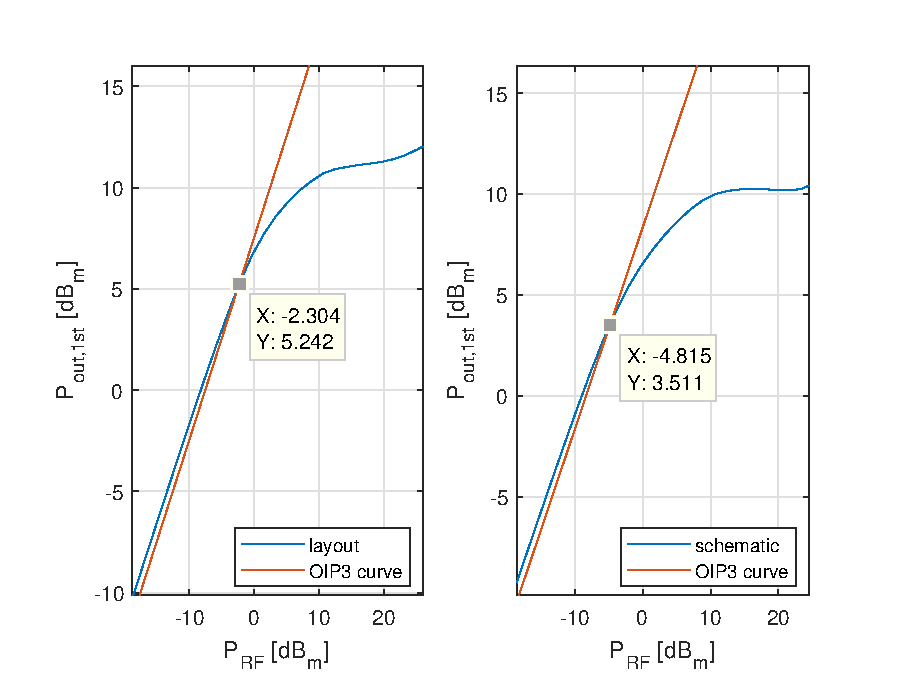
\includegraphics[width=\textwidth]{1dB_compression_1tone}
		\caption{1dB compression point, one-tone analysis}
		\label{fig:PinPout1T_1dBc}
	\end{figure}
\end{columns}
\end{frame}

\begin{frame}
\frametitle{Single tone $3^{rd}$ and $5^{th}$ order distortion}
	Increasing input power, powers of IF's $3^{rd}$ and $5^{th}$ harmonics were measured. These are in fact the first important contributions of output non-linearity. As expected from theory non-linear terms increase with the $3^{rd}$ and $5^{th}$ power of input power.
	\begin{figure}[H] 
		\centering
		\subfloat[][\emph{Harmonics power for schematic}]{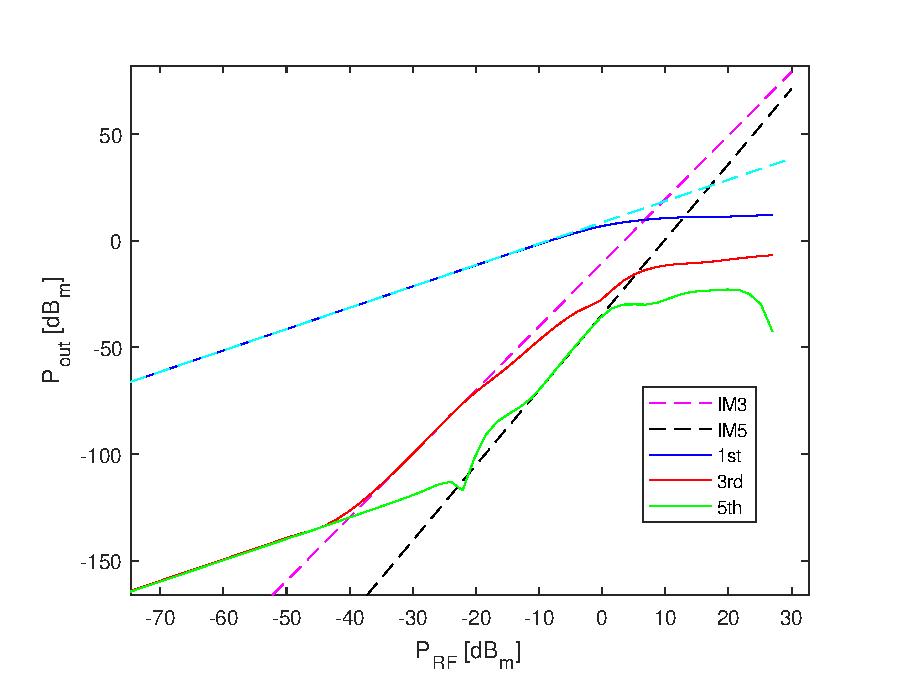
\includegraphics[width=0.5\textwidth,trim=12mm 0mm 0mm 0mm]{IIP3_schem_1tone}}
		\subfloat[][\emph{Harmonics power for layout}]{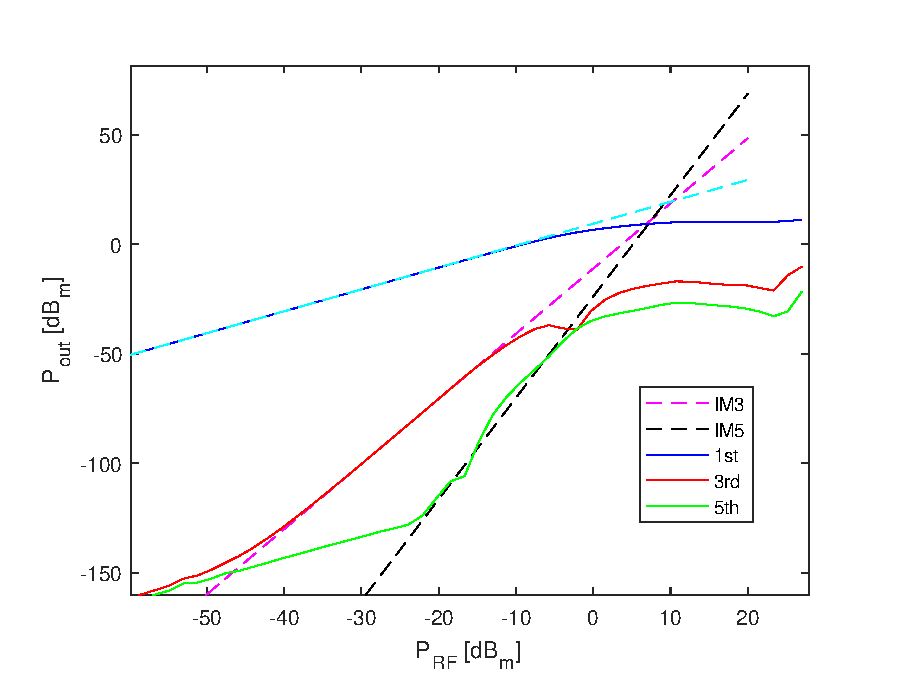
\includegraphics[width=0.5\textwidth,trim=12mm 0mm 0mm 0mm]{IIP3_layout_1tone}}
		\caption{Harmonics power, one tone analysis.}
		\label{fig:IIP3_1t_schem}
	\end{figure}
\end{frame}

\begin{frame}
\frametitle{Input and Output Intercept points}
The amount of distortion introduced can be expressed measuring the intercept points among the linear regressions of power on fundamental and the ones on harmonics. Coordinates and ordinates are called input and output intercept points (IIP3,IIP5 and OIP3,OIP5 respectively).
\begin{figure}[H] 
	\centering
	\subfloat[][\emph{Harmonics power for schematic}]{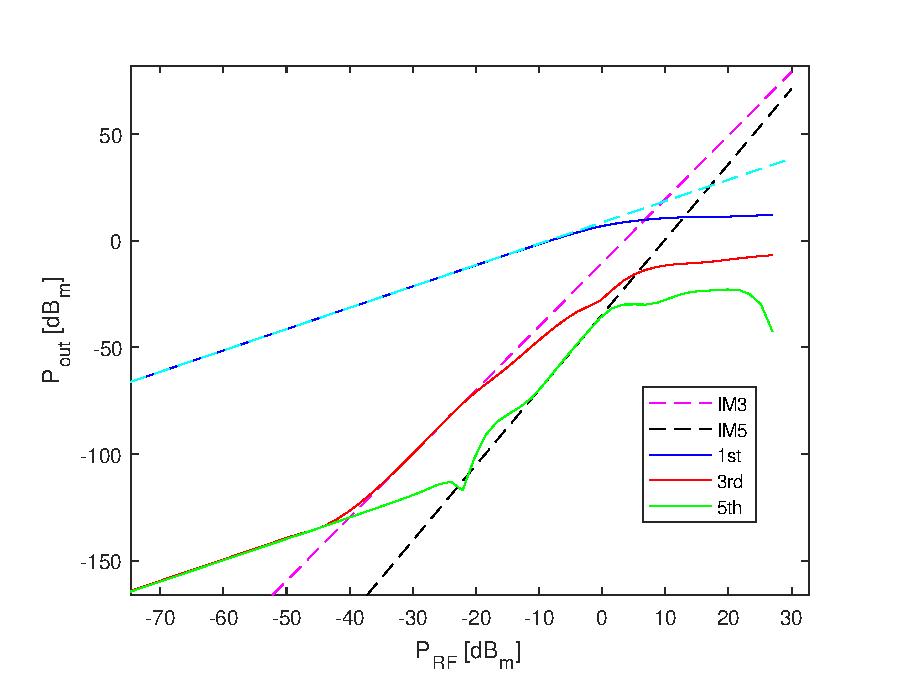
\includegraphics[width=0.5\textwidth,trim=12mm 0mm 0mm 0mm]{IIP3_schem_1tone}}
	\subfloat[][\emph{Harmonics power for layout}]{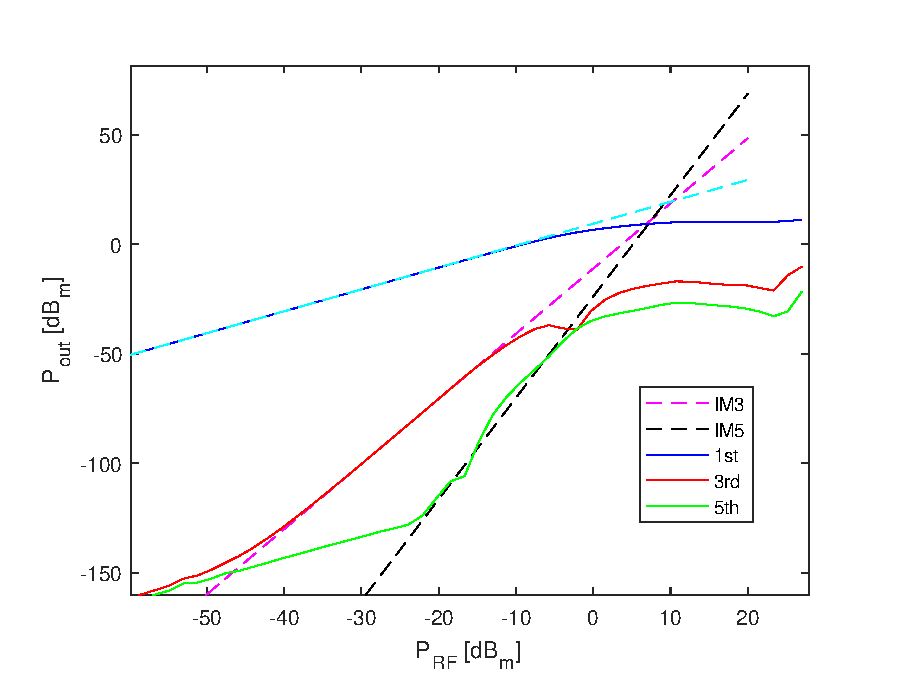
\includegraphics[width=0.5\textwidth,trim=12mm 0mm 0mm 0mm]{IIP3_layout_1tone}}
	\caption{Harmonics power, one tone analysis.}
	\label{fig:IIP3_1t_schem}
\end{figure}
\end{frame}

\begin{frame}
\frametitle{IIP3, IIP5, OIP3, OIP5}
\begin{columns}
	\column{0.5\textwidth}
	IIPs and OIPs measured are shown zooming in on the compression, and reported in table:
	\column{0.4\textwidth}
	\begin{table}[H]
		\label{tab:IIP3_1tone}
		\centering	
		\resizebox{\columnwidth}{!}{%
		\begin{tabular}{lccr} 
			\toprule 
			Parameter & Schematic 	& Layout & unit \\ 
			\midrule
			\(IIP_{3}\)  & 9.73 & 10.4 & dB\(_{m}\) \\
			\(OIP_{3}\)  & 18.3 &19.7 & dB\(_{m}\) \\
			\(IIP_{5}\)  & 17.0 &9.13 & dB\(_{m}\) \\
			\(OIP_{5}\)  & 25.6 &18.5 & dB\(_{m}\) \\
			\bottomrule 
		\end{tabular}	
	}
	\end{table}
	\end{columns}
	\begin{figure}[H] 
		\centering
		\subfloat[][\emph{Schematic detail of IPs}]{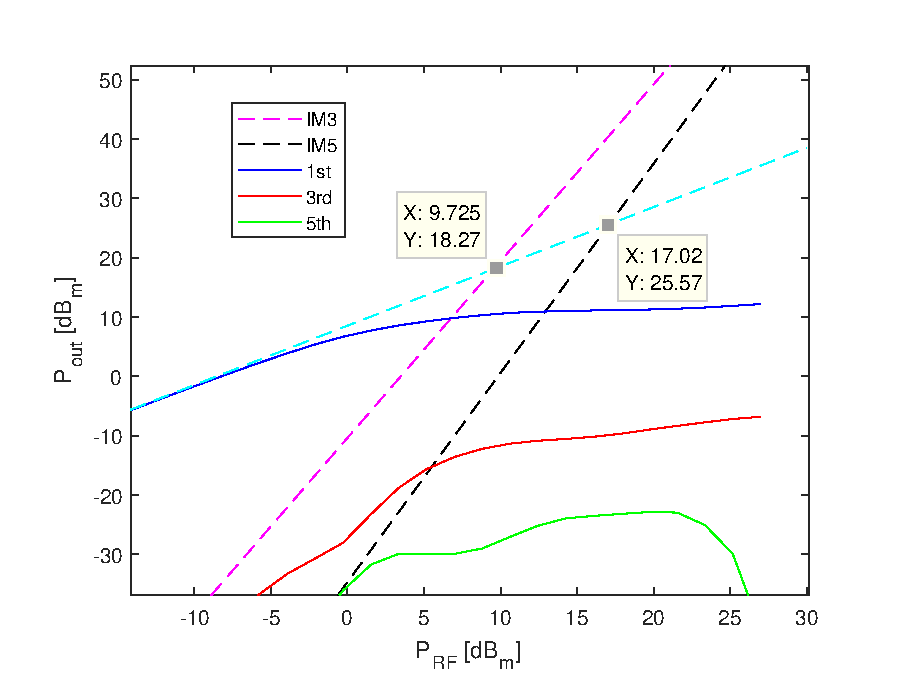
\includegraphics[width=0.5\textwidth,trim= 0mm 0mm 0mm 20mm]{IIP3_schem_1tone_zoom}}
		\subfloat[][\emph{Layout detail of IPs}]{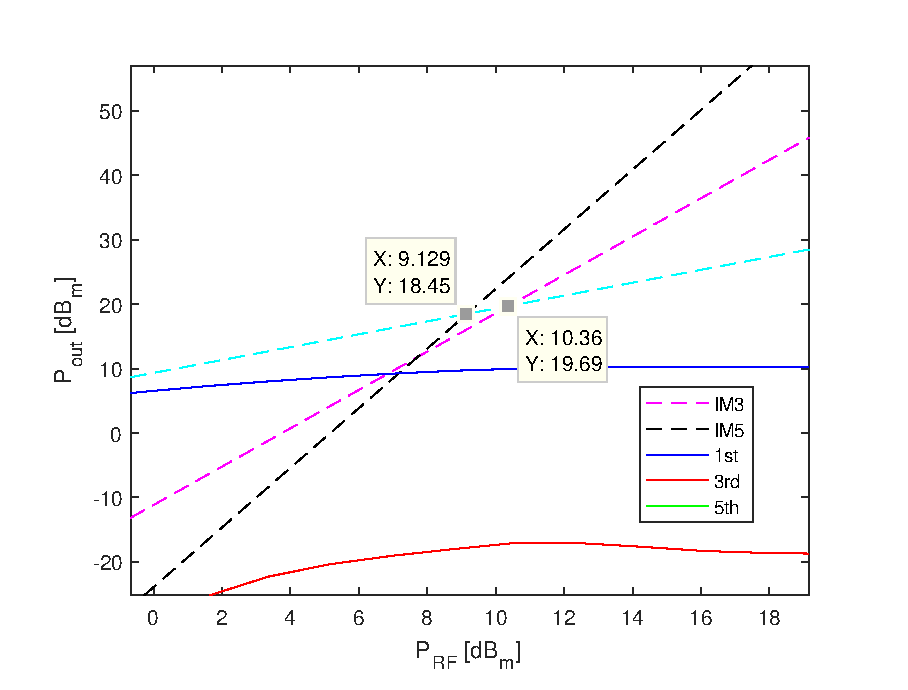
\includegraphics[width=0.5\textwidth,trim= 0mm 0mm 0mm 20mm]{IIP3_layout_1tone_zoom}}
		\label{fig:IIP3_1t_schem}
	\end{figure}
\end{frame}


\begin{frame}
\frametitle{Two tone analysis}
\begin{columns}
	\column{0.45\textwidth}
	In order to simulate a non monochrome, fixed bandwidth signal a two tone analysis was carried on. The two tones are at 110MHz and 111MHz. In-band third order intermodulation products result to be at 9MHz and 12MHz. Graphs show that power related to fundamental is strongly reduced when two tones are injected, since power is spread among all intermodulation products.
	\column{0.4\textwidth}
	\begin{figure}[H] 
		\centering
		\subfloat[][\centering\emph{schematic 1dB compression point}]{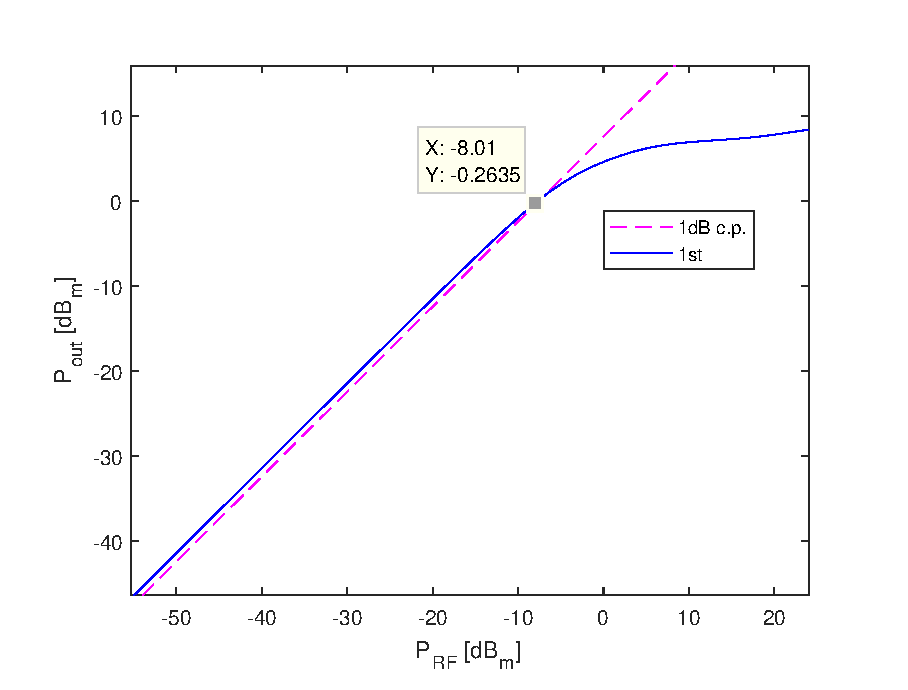
\includegraphics[height=0.3\textheight,trim=0mm 7mm 0mm 8mm, clip=true]{1dB_compression_2tone_schem}}\\
		\subfloat[][\emph{layout}]{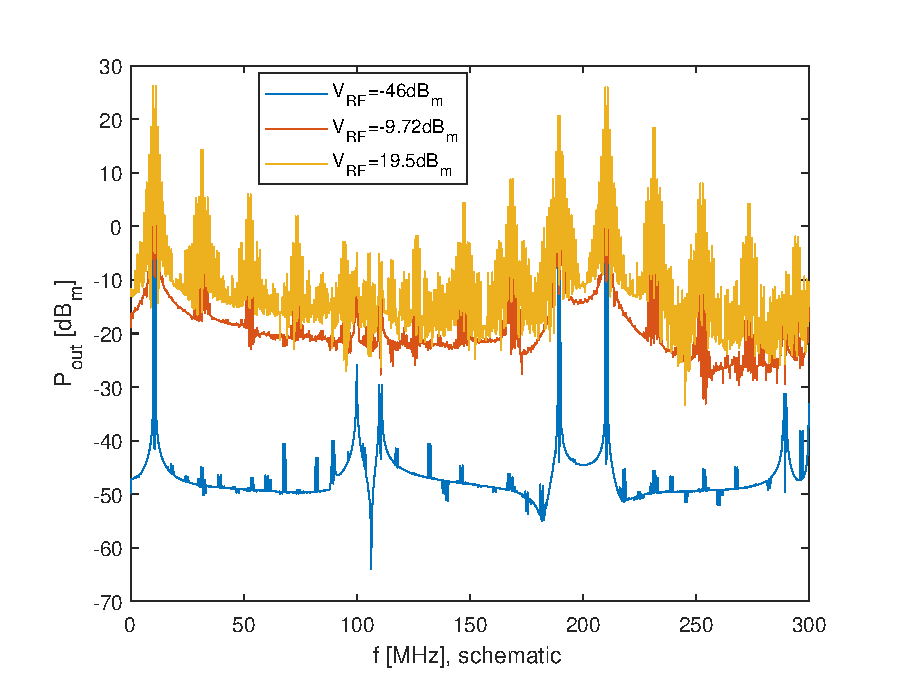
\includegraphics[height=0.3\textheight,trim=0mm 7mm 0mm 8mm, clip=true]{DFT_2tones_schem}}
		\label{fig:1dB_2tones}
	\end{figure}
\end{columns}
\end{frame}


\begin{frame}
\frametitle{Two tone analysis 1dB compression}
	Compression points for both schematic and layout.
	\begin{figure}[H] 
		\centering
		\subfloat[][\emph{schematic}]{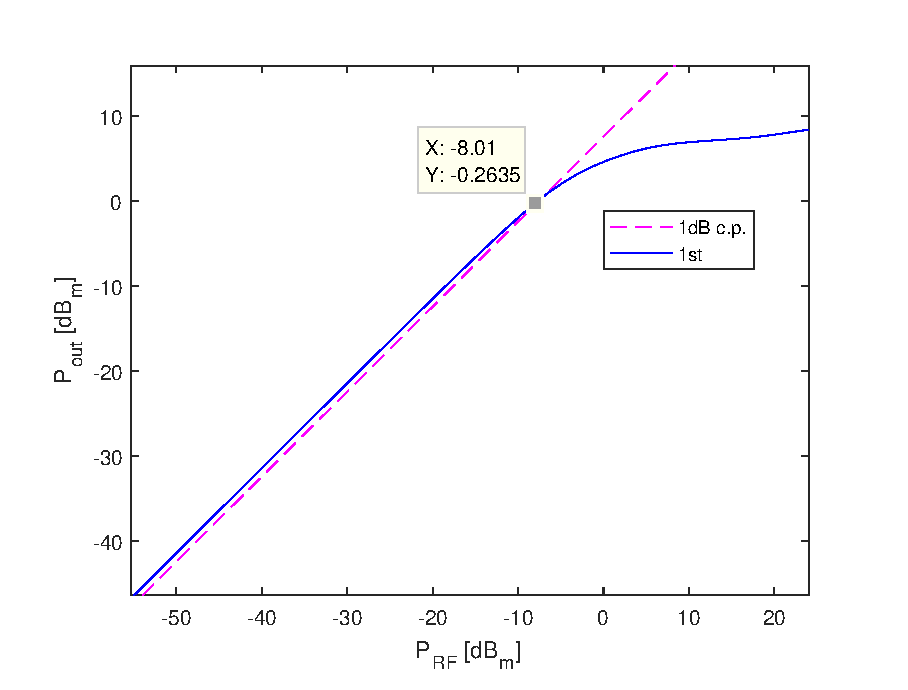
\includegraphics[width=0.5\textwidth]{1dB_compression_2tone_schem}}
		\subfloat[][\emph{layout}]{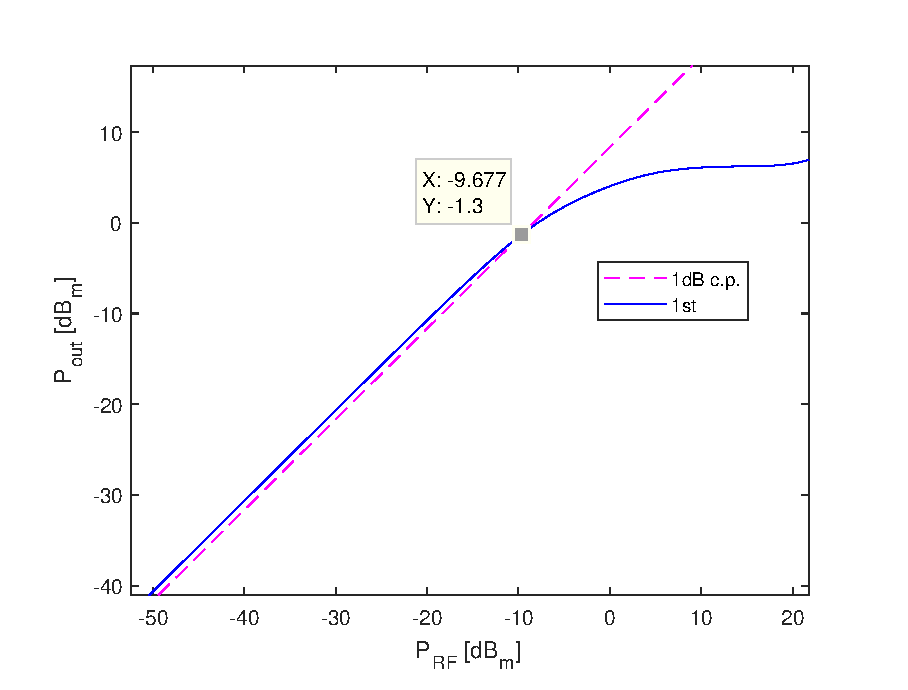
\includegraphics[width=0.5\textwidth]{1dB_compression_2tone_layout}}
		\caption{1dB compression points, two tones.}
		\label{fig:1dB_2tones}
	\end{figure}
\end{frame}


\begin{frame}
\frametitle{Two tone analysis: IM3s'IPs}
Being the power moved from the fundamental to IMPs, input and output intercepts point result lowered with respect the 1-tone case.
\begin{figure}[H] 
	\centering
	\subfloat[][\emph{schematic}]{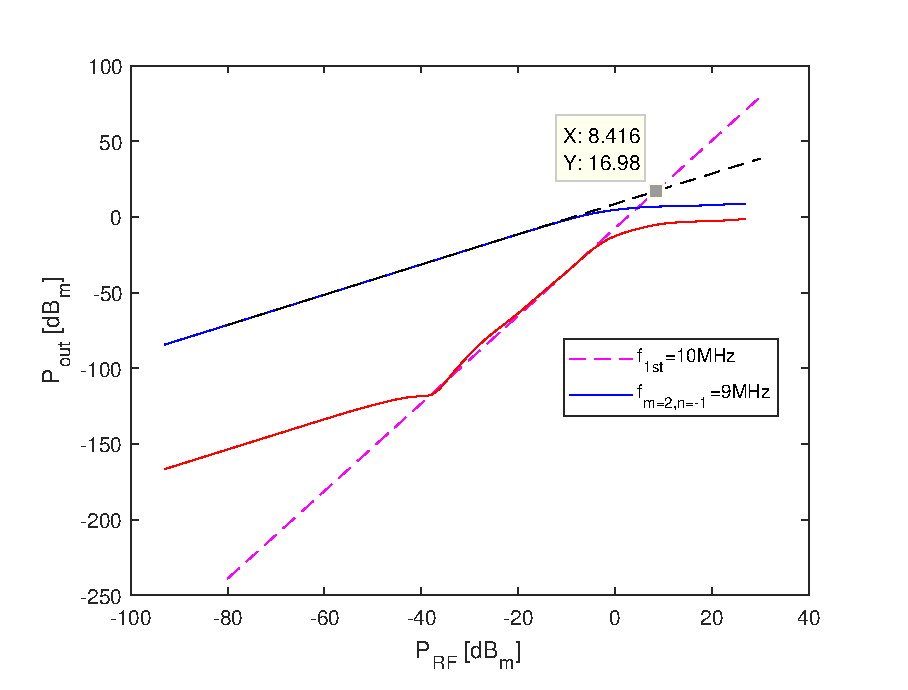
\includegraphics[width=0.5\textwidth]{IIP3_schem_2tone}}
	\subfloat[][\emph{layout}]{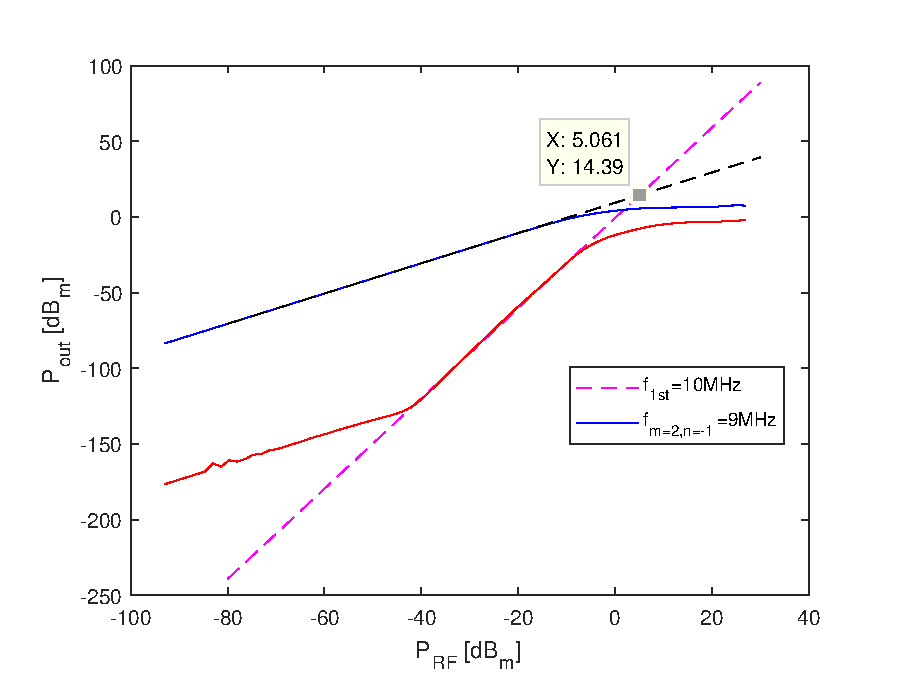
\includegraphics[width=0.5\textwidth]{IIP3_layout_2tone}}
	\caption{Harmonics power, IIP\textsubscript{3} in schematic and layout, two tone analysis.}
	\label{fig:IIP3_2t_schem}
\end{figure}
\end{frame}

\begin{frame}
\frametitle{Two tone analysis: spectra}
Frequency spectra at difference input power have been retrieved for schematic and layout. It is clearly visible the intrinsic rejection of LO and RF frequencies of the Gilbert double balanced cell.
\begin{figure}[H] 
	\centering
	\subfloat[][\emph{schematic}]{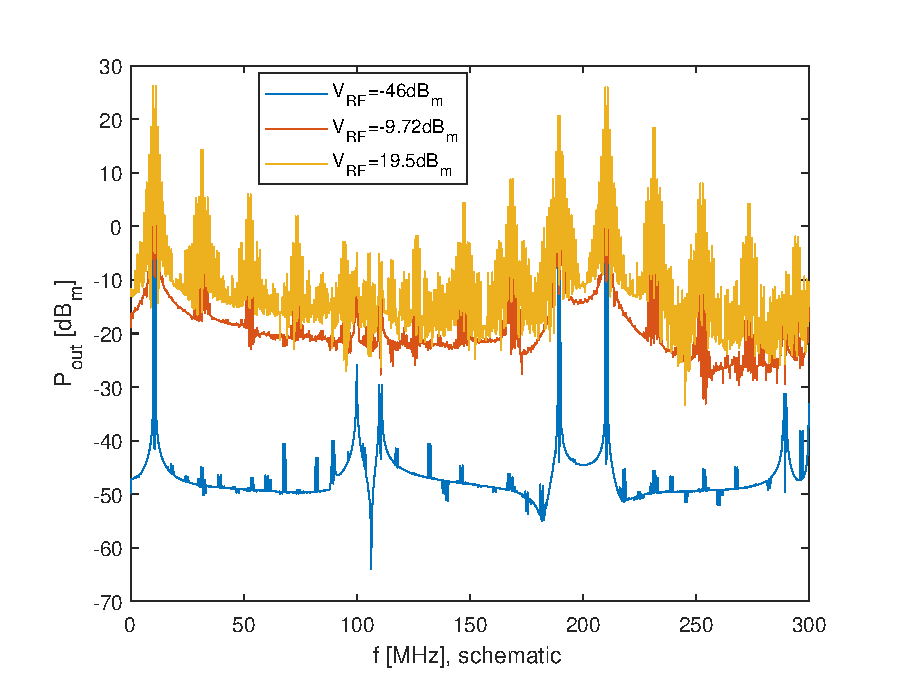
\includegraphics[width=0.5\textwidth]{DFT_2tones_schem}}
	\subfloat[][\emph{layout}]{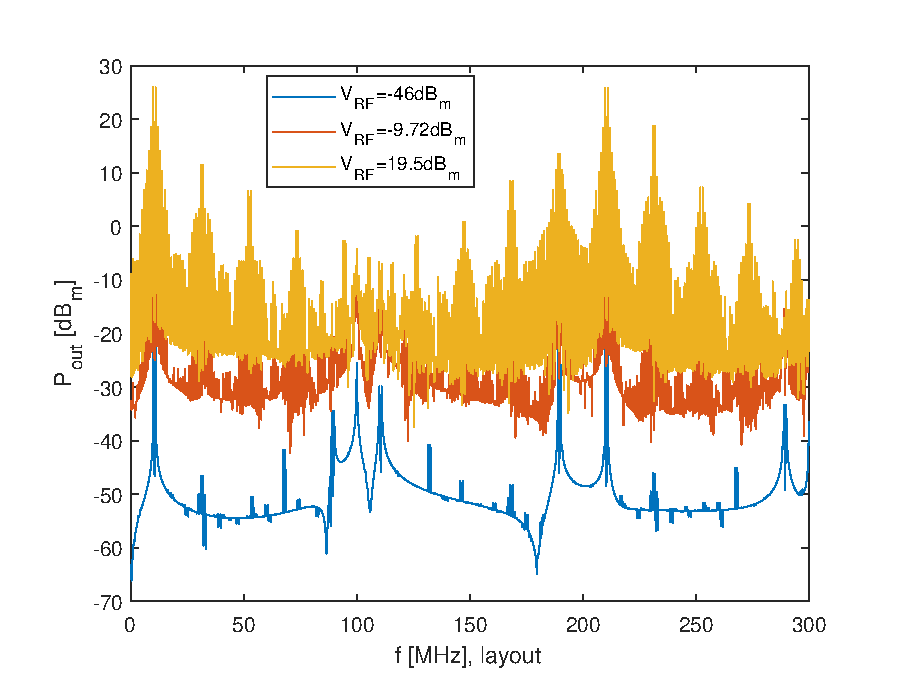
\includegraphics[width=0.5\textwidth]{DFT_2tones_layout}}
	\caption{DFT, comparison between layout and schematic; cosine2 smoothing function.}
	\label{fig:DFT_2ton}
\end{figure}
\end{frame}


\begin{frame}
\frametitle{Two tone analysis: CIM3}
The 1dB compression point spectrum has been chosen (PRF=-9.68dBm) to measure the CIM3 ratio, since this is set as the maximum input power accepted by the multiplier without heavy distortion.
\begin{figure}[H] 
	\centering
	\subfloat[][\emph{schematic}]{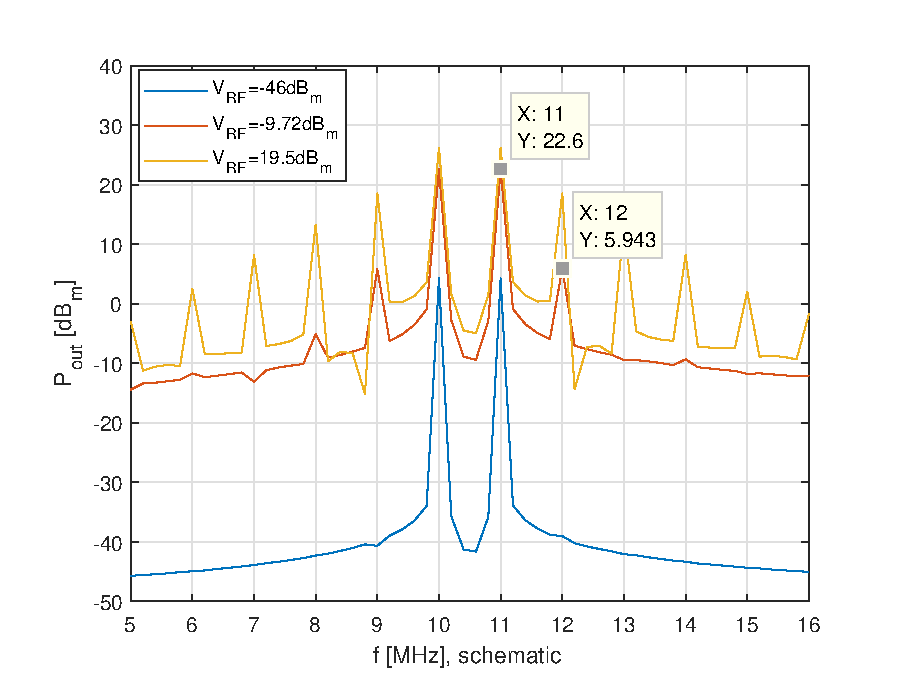
\includegraphics[width=0.5\textwidth]{DFT_2tones_schem_zoom}}
	\subfloat[][\emph{layout}]{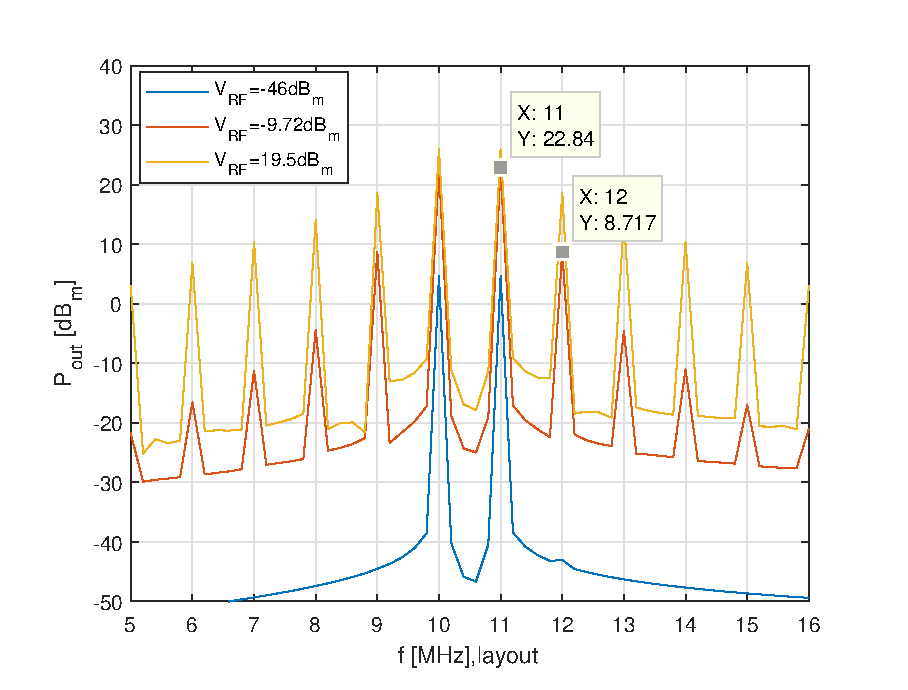
\includegraphics[width=0.5\textwidth]{DFT_2tones_layout_zoom}}
	\caption{DFT, comparison between layout and schematic. CIM\textsubscript{3} measurement at 1dB compression point; cosine2 smoothing function. }
	\label{fig:DFT_2ton_zoom}
\end{figure}
\end{frame}

\begin{frame}
\frametitle{Two tone analysis: CIM3}
As it appears, power carried from fundamental tones (10MHz and 11MHz) barely increases after this point, whereas other tones keep increasing. 
\begin{figure}[H] 
	\centering
	\subfloat[][\emph{schematic}]{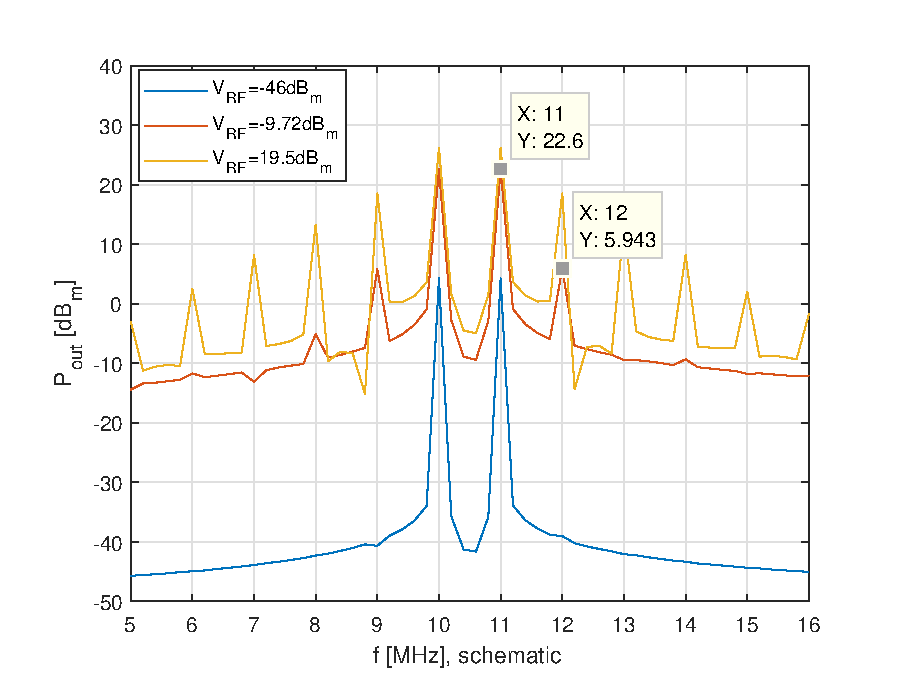
\includegraphics[width=0.5\textwidth]{DFT_2tones_schem_zoom}}
	\subfloat[][\emph{layout}]{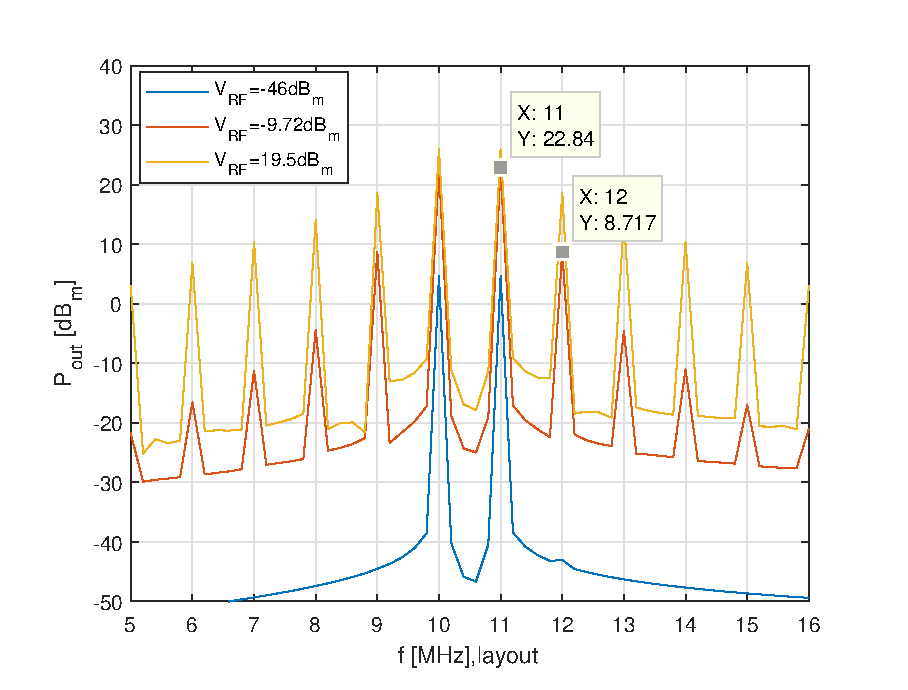
\includegraphics[width=0.5\textwidth]{DFT_2tones_layout_zoom}}
	\caption{DFT, comparison between layout and schematic. CIM\textsubscript{3} measurement at 1dB compression point; cosine2 smoothing function. }
	\label{fig:DFT_2ton_zoom}
\end{figure}
\end{frame}

\begin{frame}
\frametitle{Two tone analysis: Summing up}
The table with summarized results for the analysis is reported below. Overall, the layout looks less performing as expected. 
\begin{figure}[H] 
	\centering
	\subfloat[][\emph{schematic}]{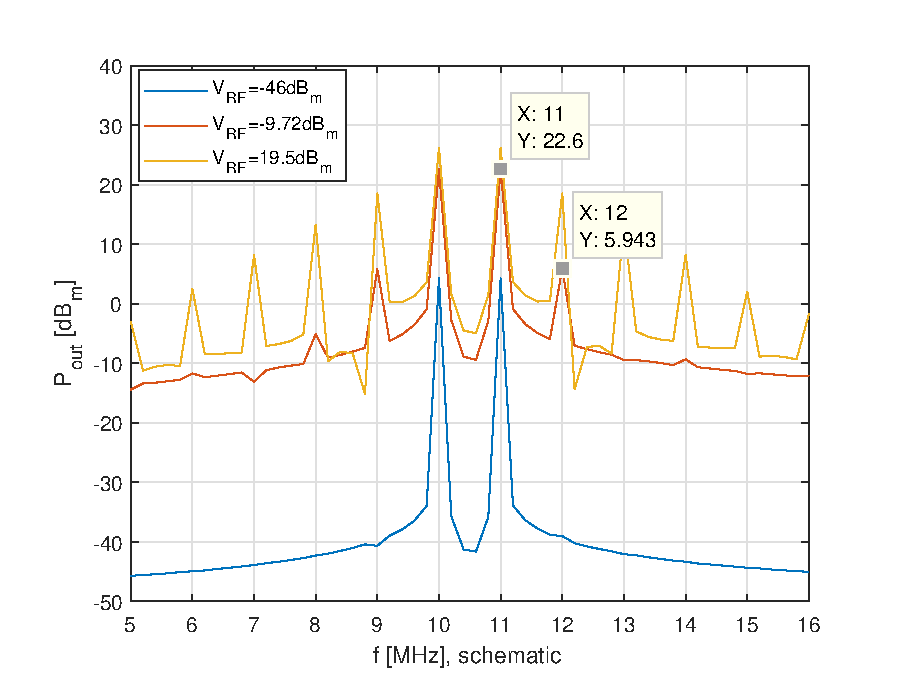
\includegraphics[width=0.5\textwidth]{DFT_2tones_schem_zoom}}
	\subfloat[][\emph{layout}]{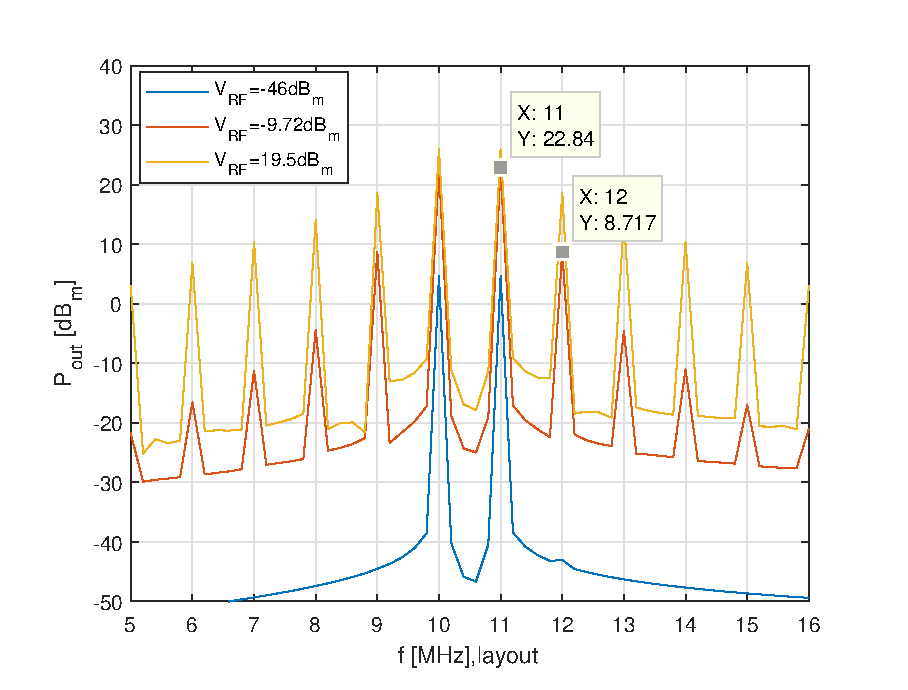
\includegraphics[width=0.5\textwidth]{DFT_2tones_layout_zoom}}
	\caption{DFT, comparison between layout and schematic. CIM\textsubscript{3} measurement at 1dB compression point; cosine2 smoothing function. }
	\label{fig:DFT_2ton_zoom}
\end{figure}
\end{frame}